\documentclass[11pt]{paper}
\usepackage{palatino}
\usepackage{amsfonts,amsmath,amssymb}
% \usepackage{graphicx}

\usepackage{listings}
\usepackage{textcomp}
\usepackage{color}

\definecolor{dkgreen}{rgb}{0,0.6,0}
\definecolor{gray}{rgb}{0.5,0.5,0.5}
\definecolor{mauve}{rgb}{0.58,0,0.82}

\lstset{frame=tb,
  language=R,
  aboveskip=3mm,
  belowskip=3mm,
  showstringspaces=false,
  columns=flexible,
  basicstyle={\small\ttfamily},
  numbers=none,
  numberstyle=\tiny\color{gray},
  keywordstyle=\color{blue},
  commentstyle=\color{dkgreen},
  stringstyle=\color{mauve},
  breaklines=true,
  breakatwhitespace=true,
  tabsize=3
}



\ifx\pdftexversion\undefined
    \usepackage[dvips]{graphicx}
\else
    \usepackage[pdftex]{graphicx}
    \usepackage{epstopdf}
    \epstopdfsetup{suffix=}
\fi

\usepackage{subfig}

\begin{document}

%%%%%%%%%%%%%%%%%%%%%%%%%%%%%%%%%%%%%%%%
% Problem Set 7
%%%%%%%%%%%%%%%%%%%%%%%%%%%%%%%%%%%%%%%%

\pagestyle{empty}
{\noindent\bf Spring 2023 \hfill Firstname M.~Lastname}
\vskip 16pt
\centerline{\bf University of Central Florida}
\centerline{\bf College of Business}
\vskip 16pt
\centerline{\bf QMB 6911}
\centerline{\bf Capstone Project in Business Analytics}
\vskip 10pt
\centerline{\bf Solutions:  Problem Set \#6}
\vskip 32pt
\noindent

\section{Data Description}

This analysis follows the script \texttt{Tractor\_Reg\_Model.R} to produce a more accurate model for used tractor prices with the data from \texttt{TRACTOR7.csv} in the \texttt{Data} folder. 
The dataset includes the following variables.
\begin{table}[h!]
\begin{tabular}{l l l}

$saleprice_i$ & = & the price paid for tractor $i$ in dollars \\
% 
$horsepower_i$ & = & the horsepower of tractor $i$ \\
$age_i$ & = & the number of years since tractor $i$ was manufactured  \\
$enghours_i$ & = & the number of hours of use recorded for tractor $i$  \\
$diesel_i$ & = & an indicator of whether tractor $i$ runs on diesel fuel \\ %, $0$ otherwise \\
$fwd_i$ & = & an indicator of whether tractor $i$ has four-wheel drive \\ %, $0$ otherwise \\
$manual_i$ & = & an indicator of whether tractor $i$ has a manual transmission \\ %, $0$ otherwise \\
$johndeere_i$ & = & an indicator of whether tractor $i$ is manufactured by John Deere \\ %, $0$ otherwise \\
$cab_i$ & = & an indicator of whether tractor $i$ has an enclosed cab \\ %, $0$ otherwise \\
% 
$spring_i$ & = & an indicator of whether tractor $i$ was sold in April or May \\ %, $0$ otherwise \\
$summer_i$ & = & an indicator of whether tractor $i$ was sold between June and September \\ %, $0$ otherwise \\
$winter_i$ & = & an indicator of whether tractor $i$ was sold between December and March \\ %, $0$ otherwise \\

\end{tabular}
\end{table}
%

I will first estimate a model with our choices of functional form, and then consider exclusions of insignificant variables from the full model. 
This approach allows for inclusion of possibly irrelevant variables and avoids excluding any relevant variables. 


%%%%%%%%%%%%%%%%%%%%%%%%%%%%%%%%%%%%%%%%
% Choosing the Dependent Variable
%%%%%%%%%%%%%%%%%%%%%%%%%%%%%%%%%%%%%%%%


\pagebreak
\section{Choosing the Dependent Variable}

Before we begin, I review the evidence for the suitability of the 
dependent variable without transformation
and compare that with the logarithmic transformation. 
Although, in this case, this decision is fairly clearly made by plotting the dependent variable alone, 
in many cases, the decision is not so clear and other forms
of evidence can be considered once building a model. 


\subsection{Univariate Analysis}

Figure \ref{fig:hist_price} shows  a histogram of tractor prices.
The distribution is highly skewed to the right, 
with most tractors selling for about \$10,000 or less,
and very few tractors priced above \$50,000.
This is a highly skewed distribution, which might influence the
estimates of parameters in the model. 


\begin{figure}[h!]
  \centering
  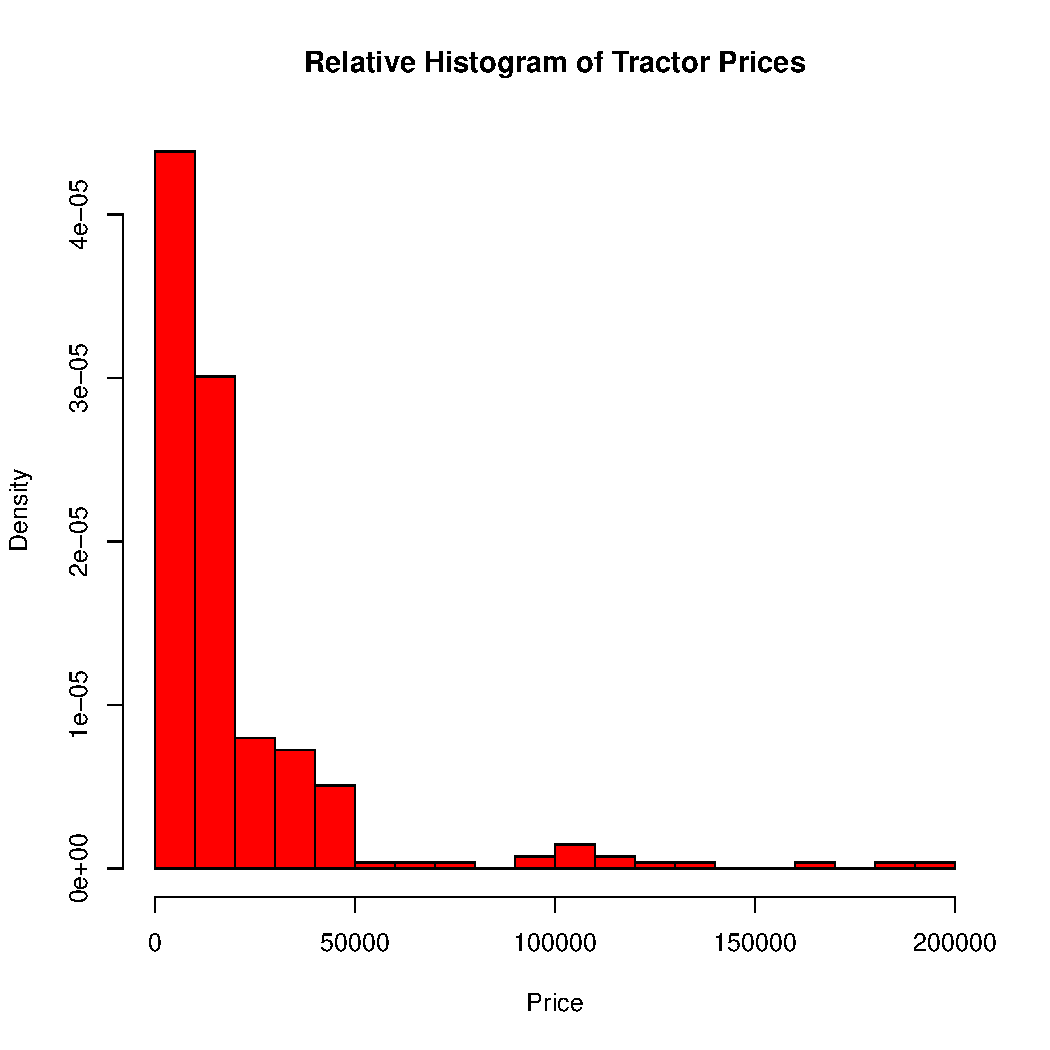
\includegraphics[scale = 0.5, keepaspectratio=true]{../Figures/hist_price}
  \caption{Histogram of Tractor Prices} \label{fig:hist_price}
\end{figure}



\pagebreak
As a comparison, Figure \ref{fig:hist_log_price} shows the histogram of the natural logarithm of
price.

\begin{figure}[h!]
  \centering
  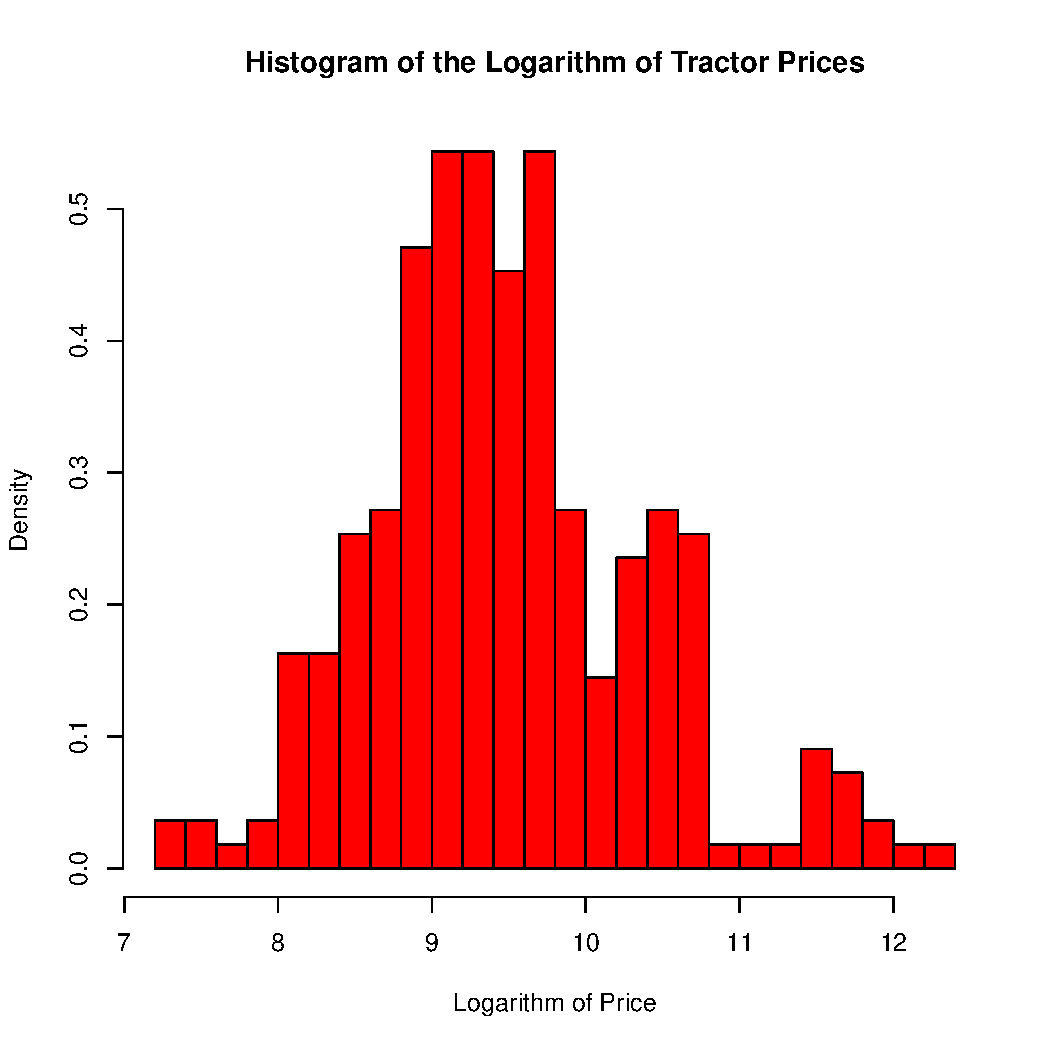
\includegraphics[scale = 0.5, keepaspectratio=true]{../Figures/hist_log_price}
  \caption{Histogram of the Logarithm of Tractor Prices} \label{fig:hist_log_price}
\end{figure}

This is much better behaved. The distribution looks almost normal. 
So far it looks as if the logarithm of the sale price
is the more promising variable.
Another approach to making this decision is
to build a model under each alternative 
and judge the validity of those results.



%%%%%%%%%%%%%%%%%%%%%%%%%%%%%%%%%%%%%%%%
% Linear Regression Models
%%%%%%%%%%%%%%%%%%%%%%%%%%%%%%%%%%%%%%%%


\pagebreak
\subsection{Linear Regression Models of Tractor Prices}

\subsubsection{Predicting Price Levels}

First, I will build a model of the price of a used tractor, 
ignoring the above evidence that the distribution is highly skewed. 


\begin{table}
\begin{center}
\begin{tabular}{l c c}
\hline
 & Prices & Log. Prices \\
\hline
(Intercept) & $11670.40884^{*}$   & $8.76953^{***}$  \\
            & $(4519.28608)$      & $(0.13528)$      \\
horsepower  & $246.39828^{***}$   & $0.00654^{***}$  \\
            & $(13.98454)$        & $(0.00042)$      \\
age         & $-674.63576^{***}$  & $-0.02754^{***}$ \\
            & $(148.99958)$       & $(0.00446)$      \\
enghours    & $-1.75752^{***}$    & $-0.00002$       \\
            & $(0.39558)$         & $(0.00001)$      \\
diesel      & $2731.97348$        & $0.49917^{***}$  \\
            & $(3996.04648)$      & $(0.11962)$      \\
fwd         & $2570.56963$        & $0.35672^{***}$  \\
            & $(2427.51242)$      & $(0.07266)$      \\
manual      & $-3713.28280$       & $-0.12167$       \\
            & $(2586.95528)$      & $(0.07744)$      \\
johndeere   & $12194.22591^{***}$ & $0.17253$        \\
            & $(2979.90884)$      & $(0.08920)$      \\
spring      & $-1721.00588$       & $-0.03210$       \\
            & $(2716.03441)$      & $(0.08130)$      \\
summer      & $-5569.45586^{*}$   & $-0.11876$       \\
            & $(2654.93625)$      & $(0.07947)$      \\
winter      & $-1541.98750$       & $0.04009$        \\
            & $(2981.31036)$      & $(0.08924)$      \\
\hline
R$^2$       & $0.64748$           & $0.69709$        \\
Adj. R$^2$  & $0.63418$           & $0.68566$        \\
Num. obs.   & $276$               & $276$            \\
\hline
\multicolumn{3}{l}{\scriptsize{$^{***}p<0.001$; $^{**}p<0.01$; $^{*}p<0.05$}}
\end{tabular}
\caption{Linear and Logarithmic Models of Tractor Prices}
\label{tab:reg_price_w_log}
\end{center}
\end{table}


The results of Model 1 in Table \ref{tab:reg_price_w_log}
shows the effect of the variables on the dollar price of the
used tractors. 

From the coefficients in the table, 
it appears that a John Deere tractor sells for 
\$12,200 more than an equivalent tractor of another brand. 
This prediction applies equally for tractors all across the spectrum, from the 
To put a finer point on it, 
a 16 horsepower lawn tractor that would otherwise sell for \$2,000 is expected to command \$14,200 if it is a John Deere.
Clearly, this is an unreasonable expectation and
a quick search on your browser will confirm that the John Deere premium is more modest. 


%\pagebreak
\subsubsection{Predicting Logarithm of Prices}

Next, I will build a model of the logarithm of the price 
of a used tractor, 
which is consistent with the univariate analysis we conducted earlier. 

% 
\begin{table}
\begin{center}
\begin{tabular}{l c}
\hline
 & Model 1 \\
\hline
(Intercept) & $8.76953^{***}$  \\
            & $(0.13528)$      \\
horsepower  & $0.00654^{***}$  \\
            & $(0.00042)$      \\
age         & $-0.02754^{***}$ \\
            & $(0.00446)$      \\
enghours    & $-0.00002$       \\
            & $(0.00001)$      \\
diesel      & $0.49917^{***}$  \\
            & $(0.11962)$      \\
fwd         & $0.35672^{***}$  \\
            & $(0.07266)$      \\
manual      & $-0.12167$       \\
            & $(0.07744)$      \\
johndeere   & $0.17253$        \\
            & $(0.08920)$      \\
spring      & $-0.03210$       \\
            & $(0.08130)$      \\
summer      & $-0.11876$       \\
            & $(0.07947)$      \\
winter      & $0.04009$        \\
            & $(0.08924)$      \\
\hline
R$^2$       & $0.69709$        \\
Adj. R$^2$  & $0.68566$        \\
Num. obs.   & $276$            \\
\hline
\multicolumn{2}{l}{\scriptsize{$^{***}p<0.001$; $^{**}p<0.01$; $^{*}p<0.05$}}
\end{tabular}
\caption{Logarithm of Tractor Prices}
\label{tab:log_price_reg_2}
\end{center}
\end{table}


The results of Model 2 in Table \ref{tab:reg_price_w_log}
shows the effect of the variables on the logarithm of the dollar price of the used tractors. 
This specification calculates coefficients that 
approximately represent percentage changes in 
tractor prices. 

From the coefficients in the table, 
it appears that a John Deere tractor sells for 
17\% more than an equivalent tractor of another brand. 
That is, a tractor worth \$1,700 would sell
for \$2,000 if it is a John Deere, 
which is clearly more reasonable. 
This more sensible interpretation supports 
the strategy of modeling the 
logarithm of the tractor price, 
even if the pricing difference is not statistically significant 
in this preliminary model. 


%%%%%%%%%%%%%%%%%%%%%%%%%%%%%%%%%%%%%%%%
\clearpage
\section{Model Specification}
%%%%%%%%%%%%%%%%%%%%%%%%%%%%%%%%%%%%%%%%

\subsection{Variable Reduction}

Next, I can refine the model by removing some explanatory variables that do not have string predictive value.
The first candidates are those with coefficients that are not statistically significant. 
The results in Table \ref{tab:reg_reduction}


\begin{table}
\begin{center}
\begin{tabular}{l c c c}
\hline
 & Model 1 & Model 2 & Model 3 \\
\hline
(Intercept) & $8.7695^{***}$  & $8.7559^{***}$  & $8.7787^{***}$  \\
            & $(0.1353)$      & $(0.1284)$      & $(0.1279)$      \\
horsepower  & $0.0065^{***}$  & $0.0066^{***}$  & $0.0065^{***}$  \\
            & $(0.0004)$      & $(0.0004)$      & $(0.0004)$      \\
age         & $-0.0275^{***}$ & $-0.0278^{***}$ & $-0.0297^{***}$ \\
            & $(0.0045)$      & $(0.0044)$      & $(0.0043)$      \\
enghours    & $-0.0000$       & $-0.0000$       & $-0.0000$       \\
            & $(0.0000)$      & $(0.0000)$      & $(0.0000)$      \\
diesel      & $0.4992^{***}$  & $0.4884^{***}$  & $0.4246^{***}$  \\
            & $(0.1196)$      & $(0.1192)$      & $(0.1118)$      \\
fwd         & $0.3567^{***}$  & $0.3492^{***}$  & $0.3416^{***}$  \\
            & $(0.0727)$      & $(0.0721)$      & $(0.0721)$      \\
manual      & $-0.1217$       & $-0.1169$       &                 \\
            & $(0.0774)$      & $(0.0773)$      &                 \\
johndeere   & $0.1725$        & $0.1858^{*}$    & $0.1707$        \\
            & $(0.0892)$      & $(0.0888)$      & $(0.0885)$      \\
spring      & $-0.0321$       &                 &                 \\
            & $(0.0813)$      &                 &                 \\
summer      & $-0.1188$       &                 &                 \\
            & $(0.0795)$      &                 &                 \\
winter      & $0.0401$        &                 &                 \\
            & $(0.0892)$      &                 &                 \\
\hline
R$^2$       & $0.6971$        & $0.6934$        & $0.6907$        \\
Adj. R$^2$  & $0.6857$        & $0.6853$        & $0.6838$        \\
Num. obs.   & $276$           & $276$           & $276$           \\
\hline
\multicolumn{4}{l}{\scriptsize{$^{***}p<0.001$; $^{**}p<0.01$; $^{*}p<0.05$}}
\end{tabular}
\caption{Models for the Log. of Tractor Prices}
\label{tab:reg_reduction}
\end{center}
\end{table}


The first column of Table \ref{tab:reg_reduction}
shows the results from the original model of
the logarithm of tractor prices in Table \ref{tab:reg_price_w_log}. 
The coefficients for seasonal indicators, 
engine hours and manual transmission are not significant.
The John Deere indicator is not significant
but since it is a key empirical question, 
so I include it, regardless. 
I removed the indicator for manual transmission
and left in the seasonal indicators;
this specification appears in the second column. 
The next column shows the model without the seasonal indicators. 
Sometimes we see an improvement in significance of
some variables with minimal loss of predictive ability
after removing the first few variables. 
%Before making any further changes, 
%I will improve the specification of the model
%by considering nonlinear specifications. 
In the fourth column, I remove the variable for the engine hours. 
% All these changes have a similar effect on the quality of the model. 
The coefficient for the value of the John Deere brand
became insignificant as the model was trimmed down. 
Still, the coefficient is consistently in the neighborhood of 16--18\%, 
which gives an indication of the value of the brand name, if only innaccurately. 
We can revisit this question after improving the quality of the model. 
For now, the best model for the full sample of tractors
is the fully-reduced Model 5.

\clearpage
\subsection{Seasonality of the Pricing of Tractors}

In the variable redulction exercise 
of Table \ref{tab:reg_reduction},
the seasonal indicators were not statistically significant individually.
%It is possible, however, that jointly, they 
%offer an improvement in prediction. 
A valid approach is to test the joint hypothesis 
of the three exclusions together with an $F$-test.
This is a more statistically rigorous way
to test the joint hypothesis that the time of year has no effect on the sale of tractors. 
%
The null hypothesis is the joint hypothesis that all coefficients on spring, summer and winter are equal to zero. 
The alternative hypothesis is that one of these coefficients is nonzero. 
% 

From the script \texttt{Tractor\_Reg\_Models.R}, the Residual Sum of Squares from the unconstrained model (the model which includes the seasonal indicators) is $41.78944$. 
The constrained model is the one that excludes seasonal indicators and it has a Residual Sum of Squares of $42.15882$.

The $F$-statistic has a value of 

$$ 
\frac{(RSS_M - RSS)/M}{RSS/(N - K)} = \frac{(67.17639 - 66.40924)/3}{RSS/263} = 1.024257. 
$$

since $N = 276$ observations, $K = 10$ variables and $M = 3$ restrictions, one for each seasonal indicator excluded. 
This is a low value compared to the critical value of $2.60$ for the $F$-statistic with $3$ degrees of freedom in the numerator and $263 (> 120)$ degrees of freedom in the denominator. 
There is no evidence to reject the null that all seasonal indicators have coefficients of zero and we conclude that the seasonal indicators should be left out of the model. 
%
The results of the test above coincide with the conclusion drawn from
the individual $t$-statistics:
both indicate that tractor prices do not follow a seasonal pattern. 


\clearpage
\subsection{Interaction Terms}


%\subsubsection{Durability of Engine Types}
%
%Finally, I consider another modification to your model. 
%Diesel engines tend to be more durable than gasoline engines. 
%This raises the question of whether an additional hour of use affects the value of a diesel tractor differently than for a gasoline tractor. 
%This is tested in Model 1 of Table \ref{tab:reg_interactions}. 
%
%	This hypothesis is a test of the \emph{interaction} of the diesel indicator and the slope on engine hours. 
%      Given the above result, this test should be conducted with the model that excludes the seasonal indicators. 
%The coefficient on \texttt{enghours:diesel} is $5.882e-06$ with a standard error of $2.922e-05$, resulting in a $t$-statistic of $0.201$. 
%Since this is a very low value, we cannot reject the null hypothesis that an additional hour of use affects the value of a diesel tractor the same as that for a gasoline tractor. 
%Note that this conclusion does not change if you test a one-sided hypothesis.  
%
%Furthermore, the $\bar{R}^2$ statistic decreases with the inclusion of this variable. 
%The $F$-statistic is high and statistically significant, indicating that this model is better than the simple average but so is the model without this new variable. 
%Finally, the estimates of the other coefficients change very little when this variable is omitted. 
%The theory may be sound but there is nothing else to support the inclusion of this new variable. 

\subsubsection{Differences in Parameters by Brand}

The columns of Table \ref{tab:reg_interactions}
show the results of tests for interactions
between the John Deere indicator variable
on the effects of horsepower, engine hours, age
and whether the tractor has a manual transmission. 
There seems to be no evidence for relationships that differ by
brand name. 


\begin{table}
\begin{center}
\begin{tabular}{l c c c c}
\hline
 & Model 1 & Model 2 & Model 3 & Model 4 \\
\hline
(Intercept)          & $8.89189^{***}$  & $8.88028^{***}$  & $8.87926^{***}$  & $8.89127^{***}$  \\
                     & $(0.12827)$      & $(0.11042)$      & $(0.11163)$      & $(0.11165)$      \\
horsepower           & $0.00488^{***}$  & $0.00490^{***}$  & $0.00489^{***}$  & $0.00476^{***}$  \\
                     & $(0.00039)$      & $(0.00039)$      & $(0.00039)$      & $(0.00043)$      \\
age                  & $-0.02986^{***}$ & $-0.02994^{***}$ & $-0.02990^{***}$ & $-0.02969^{***}$ \\
                     & $(0.00381)$      & $(0.00381)$      & $(0.00400)$      & $(0.00381)$      \\
enghours             & $-0.00004$       & $-0.00004^{***}$ & $-0.00004^{***}$ & $-0.00004^{***}$ \\
                     & $(0.00003)$      & $(0.00001)$      & $(0.00001)$      & $(0.00001)$      \\
diesel               & $0.28447^{*}$    & $0.30271^{**}$   & $0.29874^{**}$   & $0.29293^{**}$   \\
                     & $(0.12619)$      & $(0.10378)$      & $(0.10389)$      & $(0.10387)$      \\
fwd                  & $0.25952^{***}$  & $0.25727^{***}$  & $0.25879^{***}$  & $0.26050^{***}$  \\
                     & $(0.06238)$      & $(0.06230)$      & $(0.06229)$      & $(0.06226)$      \\
manual               & $-0.16119^{*}$   & $-0.15793^{*}$   & $-0.16018^{*}$   & $-0.16217^{*}$   \\
                     & $(0.06631)$      & $(0.06632)$      & $(0.06692)$      & $(0.06619)$      \\
johndeere            & $0.31091^{***}$  & $0.25824^{*}$    & $0.30345^{*}$    & $0.24957^{*}$    \\
                     & $(0.07868)$      & $(0.11399)$      & $(0.15228)$      & $(0.10998)$      \\
cab                  & $0.67506^{***}$  & $0.67717^{***}$  & $0.67571^{***}$  & $0.67665^{***}$  \\
                     & $(0.06732)$      & $(0.06728)$      & $(0.06734)$      & $(0.06722)$      \\
enghours:diesel      & $0.00001$        &                  &                  &                  \\
                     & $(0.00003)$      &                  &                  &                  \\
enghours:johndeere   &                  & $0.00001$        &                  &                  \\
                     &                  & $(0.00002)$      &                  &                  \\
age:johndeere        &                  &                  & $0.00023$        &                  \\
                     &                  &                  & $(0.00742)$      &                  \\
horsepower:johndeere &                  &                  &                  & $0.00057$        \\
                     &                  &                  &                  & $(0.00077)$      \\
\hline
R$^2$                & $0.77769$        & $0.77795$        & $0.77766$        & $0.77811$        \\
Adj. R$^2$           & $0.77017$        & $0.77043$        & $0.77014$        & $0.77060$        \\
Num. obs.            & $276$            & $276$            & $276$            & $276$            \\
\hline
\multicolumn{5}{l}{\scriptsize{$^{***}p<0.001$; $^{**}p<0.01$; $^{*}p<0.05$}}
\end{tabular}
\caption{Regression Models for Tractor Prices}
\label{tab:reg_interactions}
\end{center}
\end{table}



\clearpage
\pagebreak
\subsubsection{Separate Models by Brand}

In Table \ref{tab:reg_interactions}, 
we investigated several 
individual types of differences by brand. 
To test for many possible differences in 
models by brand of tractor, 
Table \ref{tab:reg_johndeere}
shows the estimates for two separate models
by brand of tractor.
%
Model 1 shows the estimates for 
the full sample,
Models 2, 3 and 4 show the estimates from two models for 
John Deere tractors
and Models 5 and 6 
represent all other brands. 
% 
Models 3 and 5 show the estimates from 
the best, reduced version of each model, 
in which all coefficients are statistically significant. 
% 
The coefficients appear similar across the two subsamples, 
when the coefficients are significant.
Notable differences include the statistical significance for 
the indicators for four-wheel drive, 
manual transmission and an enclosed cab. 
These features seem to change the value of 
other tractors, but perhaps these coefficients are not measured 
accurately for the small sample of 39 
John Deere tractors. 


\begin{table}
\begin{center}
\begin{tabular}{l c c c c c}
\hline
 & Model 1 & Model 2 & Model 3 & Model 4 & Model 5 \\
\hline
(Intercept)         & $8.72792^{***}$  & $8.86706^{***}$  & $9.03796^{***}$  & $8.77320^{***}$  & $8.90792^{***}$  \\
                    & $(0.10602)$      & $(0.22409)$      & $(0.16430)$      & $(0.12450)$      & $(0.08769)$      \\
horsepower          & $0.01112^{***}$  & $0.01502^{***}$  & $0.01580^{***}$  & $0.01032^{***}$  & $0.01057^{***}$  \\
                    & $(0.00107)$      & $(0.00250)$      & $(0.00223)$      & $(0.00119)$      & $(0.00119)$      \\
squared\_horsepower & $-0.00001^{***}$ & $-0.00002^{***}$ & $-0.00002^{***}$ & $-0.00001^{***}$ & $-0.00001^{***}$ \\
                    & $(0.00000)$      & $(0.00000)$      & $(0.00000)$      & $(0.00000)$      & $(0.00000)$      \\
age                 & $-0.03233^{***}$ & $-0.03038^{**}$  & $-0.03295^{***}$ & $-0.03164^{***}$ & $-0.03283^{***}$ \\
                    & $(0.00358)$      & $(0.00914)$      & $(0.00738)$      & $(0.00399)$      & $(0.00392)$      \\
enghours            & $-0.00004^{***}$ & $-0.00006^{*}$   & $-0.00006^{**}$  & $-0.00004^{***}$ & $-0.00004^{***}$ \\
                    & $(0.00001)$      & $(0.00002)$      & $(0.00002)$      & $(0.00001)$      & $(0.00001)$      \\
diesel              & $0.20350^{*}$    & $0.08485$        &                  & $0.18218$        &                  \\
                    & $(0.09805)$      & $(0.18242)$      &                  & $(0.11984)$      &                  \\
fwd                 & $0.26539^{***}$  & $0.12882$        &                  & $0.29072^{***}$  & $0.30003^{***}$  \\
                    & $(0.05820)$      & $(0.15529)$      &                  & $(0.06308)$      & $(0.06296)$      \\
manual              & $-0.15015^{*}$   & $0.06749$        &                  & $-0.17919^{**}$  & $-0.14668^{*}$   \\
                    & $(0.06189)$      & $(0.17288)$      &                  & $(0.06743)$      & $(0.06413)$      \\
johndeere           & $0.31872^{***}$  &                  &                  &                  &                  \\
                    & $(0.07186)$      &                  &                  &                  &                  \\
cab                 & $0.48345^{***}$  & $0.32344$        & $0.38517^{*}$    & $0.51732^{***}$  & $0.52756^{***}$  \\
                    & $(0.07003)$      & $(0.17555)$      & $(0.16365)$      & $(0.07696)$      & $(0.07688)$      \\
\hline
R$^2$               & $0.80591$        & $0.91993$        & $0.91606$        & $0.77992$        & $0.77769$        \\
Adj. R$^2$          & $0.79935$        & $0.89858$        & $0.90334$        & $0.77220$        & $0.77090$        \\
Num. obs.           & $276$            & $39$             & $39$             & $237$            & $237$            \\
\hline
\multicolumn{6}{l}{\scriptsize{$^{***}p<0.001$; $^{**}p<0.01$; $^{*}p<0.05$}}
\end{tabular}
\caption{Separate Models by Brand}
\label{tab:reg_johndeere}
\end{center}
\end{table}


We can also test for all of the differences at the same time
by using an $F$-test. 
We do so using a comparison between the best models
for each subsample and the best model for the full sample.
In this case, the full, unrestricted model has 
% $K = 2\times9 = 18$
$K = 4 + 8 = 12$
parameters, 
one for each variable in the two models, including the intercepts. 
The test that all of the coefficients are the same has 
% $M = 9 - 1 = 8$
$M = 12 - 5 = 7$
restrictions, 
since the reduced model on the full sample has 5 parameters. 
The one restriction fewer accounts for the John Deere indicator
in the full model, 
which allows for two separate intercepts. 
% 
The $F$-statistic has a value of 

$$ 
\frac{(RSS_M - RSS)/M}{RSS/(N - K)} = \frac{(68.97084 - 48.38915)/7}{48.38915/264} = 16.04128. 
$$

%This is also a very low value for the $F$-statistic. 
%There is no evidence to reject the null that all 
%coefficients are equal across both samples 
%and conclude that the John Deere indicator
%should be the only brand difference left in the model. 
This is a very high value for the $F$-statistic. 
This is evidence to reject the null that all 
coefficients are equal across both samples 
and conclude that 
several parameters should be estimated separately
depending on whether the tractor was made by John Deere .
% the John Deere indicator
% should be the only brand difference left in the model. 

%%%%%%%%%%%%%%%%%%%%%%%%%%%%%%%%%%%%%%%%
\end{document}
%%%%%%%%%%%%%%%%%%%%%%%%%%%%%%%%%%%%%%%%
